\documentclass{article}
\usepackage[round]{natbib}
\usepackage{amsmath,amssymb,amsfonts, bbm}%
\usepackage{geometry}%
\usepackage{color}
\usepackage{graphicx}
\usepackage{authblk}
\usepackage{nameref}
\usepackage[right]{lineno}
\usepackage{subcaption}
\usepackage{tikz}

\newcommand{\tsinfer}[0]{\texttt{tsinfer}}
\newcommand{\kwarg}[0]{\texttt{KwARG}}
\newcommand{\argweaver}[0]{\texttt{ARGweaver}}
\newcommand{\argweaverD}[0]{\texttt{ARGweaver-D}}
\newcommand{\relate}[0]{\texttt{Relate}}
\newcommand{\espalier}[0]{\texttt{Espalier}}
\newcommand{\arbores}[0]{\texttt{Arbores}}
\newcommand{\tskit}[0]{\texttt{tskit}}

% Bold the 'Figure #' in the caption and separate it from the title/caption with a period
% Captions will be left justified
\usepackage[aboveskip=1pt,labelfont=bf,labelsep=period,justification=raggedright,singlelinecheck=off]{caption}
\renewcommand{\figurename}{Fig}

% deal with supplementary items
\newcommand{\supplementarysection}{%
  \setcounter{figure}{0}% Reset figure counter
  \let\oldthefigure\thefigure% Capture figure numbering scheme
  \renewcommand{\thefigure}{S\oldthefigure}% Prefix figure number with S
  \section{Supplementary section}% Set supplementary section
}

\begin{document}

\linenumbers
\title{Computing likelihoods under the SMC for a general class of ARGs.}

% First authors
\author[1, $\dagger$]{Gertjan Bisschop}

% Middle Authors
\author[2]{Alison Etheridge}
\author[3]{Peter Ralph}

% last author
\author[1]{Jerome Kelleher}
\affil[$\dagger$]{Denotes corresponding author}

\maketitle

\affil[1]{Big Data Institute, Li Ka Shing Centre for Health Information and Discovery, University of Oxford, OX3 7LF, UK}
\affil[2]{Department of Statistics, University of Oxford, OX1 3LB, UK}
\affil[3]{University of Oregon, USA}

\section{Abstract}
This means there currently is no way to connect the output of the diverse 
range of ARG inference methods back 
to a model that would allow us to perform a probabilistic exploration of the 
ARG space around the point estimate, or likelihood-based inference

\section{Introduction}

[great point from Wong et al] Note that it is important to distinguish 
here between structures and models: whether an inference method is based on 
heuristics or a rigorous mathematical model is orthogonal to the level 
of detail provided in its estimate. One could heuristically estimate a 
fully precise ARG, or statistically sample a partial, approximate ARG under 
a model such as the coalescent.
What we want to achieve with this paper is to bring the two concepts closer 
to each other. Compute a likelihood for an approximate (define) ARG under a 
approximate model of the coalescent. 
Approximate in two senses: SMC + leave out precise recombination time info


The underlying genealogical history that relates a sample of individuals back in time
contains all possible information this sample can provide on the history of demography, 
selection and recombination for the population of interest. 
Reconstructing these genealogies with certainty is impossible however. 
As such, in the past the data structure capturing these inheritance paths 
or Ancestral Recombination Graph (ARG), has usually been considered a nuisance 
variable to be integrated out during statistical inference 
\citep{kuhner_2000, griffiths_ancestral_1996}.


The breakthroughs in scale achieved by recent methods 
are all based, in different ways, on inferring approximate 
structures instead of a complete and fully detailed history
% in particular with respect to recombination nodes

% first major step forwards in ARG inference
% explicitly outputs an ARG
ARGweaver, generates these ARGs explicitly again using MCMC sampling, by discretizing time 
they can apply HMM-based algorithms to efficiently generate new samples from the distribution of 
possible ARGs.
% [TO ADD] also argweaver is the first to compute likelihoods for an ARG under the SMC, musn't forget to include this.
% model-based approaches vs 

% recent advancements: heuristics
Recently, major advancements relying on heuristic rather than model-based approaches
have made ARG inference scalable.
\citep{rasmussen_2014, kelleher_2019, speidel_2019, schaefer_2021, wohns_2022, 
zhang_biobank-scale_2023, zhan_towards_2023}. These methods
have raised the realistic prospect of ARG-based analysis becoming a standard 
part of the population and statistical genetics toolkit.
This has also meant however that
we are now using the term ARG for a varying range of approximate structures
as generated by these different inference methods \citep{wong_a-general_2023}. 
Besides not having a unified output format, The degree of completeness 
in which genetic inheritance from ancestors to 
descendants is documented by each of these methods varies extensively. 
[TO DO:] discuss: each of these tools will deal with or resolve uncertainty 
in a different way.
This has complicated the ability to connect the output of this diverse range of 
ARG inference methods to a model-based deescription that would allow us to perform  
probabilistic exploration of the ARG space around the point estimate, 
or likelihood-based inference (that does not just consider individual marginal trees).\\

Recombination in particular:
In contrast to model-based inference methods like \argweaver, 
these models only deal with recombination in an implicit sense.\\


[TO DO:] what does *general* mean? and when in the paper do we discuss it?

[TO DO: finish this section] For example, where ARGweaver has 
the built in assumption of neighbouring trees being separated by single Subtree Prune 
Regraft (SPR) [REF Song et al.], this is not the case for any of the heuristic data 
structures.
Lack recombination nodes in the ARG, crucial in ability to compute likelihoods 
under Hudson. \citep{wong_a-general_2023}




% then onto the SMC
[TO ADD: discuss SMC] mention the SMC \citep{mcvean_approximating_2004}.
SMC and relatives are useful: lot of focus however on integrating over 
the distribution of trees to get $N_e(t)$ [ADD REF: PSMC, MSMC]
Here, the idea is to use the SMC in a different way that resonates more 
with the true direction of flow of genetic information.

Results in a concrete way to compute likelihoods for *any* inferred ARG 
by integrating out the time to recombination.
and formulate an algorithm 
that is general in the sense that it can deal with the various levels of 
completeness that characterise the field's currents attempts [TO DO: make this sound more positive] 
at reconstucting genome-wide genealogies.


\section{Methods and Results}
\subsection{SMC backwards-in-time}\label{par:description}

Formulated backwards-in-time, the SMC \citep{mcvean_approximating_2005} only requires a 
simple modification to the 
coalescent with recombination. By only considering those pairs of 
lineages that share 
genomic intervals with ancestral material, as eligible for coalescence, we obtain the 
sequential Markovian structure along the chromosome.\\

More formally, and following the notation of \citet{mcvean_approximating_2005}, at any 
point in time, the process can be described by $L(t)$, the set of labeled lineages 
extant at time $t$ each represented by a union of ordered non-overlapping half open 
intervals detailing the ancestral material 
carried by that lineage $X_i = \{[x_{i0}, y_{i0}), \dotsc, [x_{im}, y_{im})\}$.
$L(0)$ consists of $n$ sampled lineages, labelled $0$ to $n-1$, each represented by a 
single interval spanning the entire genome.
Backwards in time the process evolves by a succession of coalescence and recombination 
events until each segment of ancestral material is only present in one lineage. 
The waiting time to next event is determined by these two competing processes 
with exponentially distributed waiting times as outlined below.\\

Recombination is described by a Poisson process of rate $r$ per unit of length and time. 
A recombination to the 
left of $x$ with $x>x_{i0}$ and $x<y_{im}$ splits a lineage $i$ into two new, uniquely 
labelled lineages.\\

Any two \emph{overlapping} lineages coalesce at rate $\lambda = 1/(2N_e)$ in the case
of a diploid population of constant size. The newly formed lineage acquires the 
union of both ordered intervals.
Although coalescence is reciprocal, here we'll define a strict total order 
(see \ref{par:liks}) on 
all lineages in $X(t)$ based on their leftmost starting points. 
For any such strict total order on $X(t)$ and at any point in the process 
the instantaneous rate of coalescence then equals $\lambda \sum_{i \neq j} I_{ij}$.

\begin{equation} \label{def:coal}
I_{ij} = \begin{cases}
1 & X_i > X_j \wedge X_i \cap X_j \neq \emptyset \\
0 & \text{otherwise}
\end{cases}
\end{equation}

We can now define $C_i(t) = \{X_j \in L(t) | I_{ij}(t) = 1\}$ such that $|C_i(t)| = 
I_{i}(t) = \sum_{j} I_{ij}(t)$.
Because $I_{ij}$ is not reciprocal, each extant lineage has their own unique set of 
lineages $C_i(t)$ it can coalesce with. This will simplify the likelihood computations 
(see \ref{par:liks}). Note that although recombination affects $C_i(t)$ it does not 
affect $I_{i}$.\\ 

% note on the disjoint set of intervals for each lineage under the SMC
As noted by \cite{mcvean_approximating_2005}, the backwards-in-time description of the 
SMC is slightly different from the left-to-right approach in that recombination 
in non-ancestral material is possible (see fig.\ref{fig:smc-unary}). 
Although this does not affect the distribution 
of marginal genealogies, it does mean that not all lineages in $L$ can be represented 
by a single interval. More precisely, all lineages will be associated with 
a single interval up to the point where one section of the 
genome has reached its most recent common ancestor but the neighbouring parts have not.

\subsection{Recording an ARG} \label{par:recording}

The process described in the previous paragraph details the transitions of the 
set of labeled lineages $L$ through time. An Ancestral Recombination Graph 
$\mathcal{G} = (N, E)$ capturing the various inheritance paths along the genome 
is obtained by registering an edge represented by a tuple $(c, p, X_{cp})$ 
whenever a lineage $c$, associated with a disjoint set of genomic intervals $X_c$, is 
replaced by one or two lineage(s), $p$ (and $p^{\prime}$), 
in case of a coalescence or recombination respectively.
The last element of the tuple is the extent of the edge. It is itself a  
disjoint set of intervals such that $X_{cp} \cup X_{cp^{\prime}} = X_c$. 
The set of edges $E$, containing all such tuples $(c, p, X_{cp})$, 
and $N$, the set of nodes representing all genomes in the ARG, together
define this data structure.\\

The ARG as described here records the impact of every possible event along each 
inheritance path in full detail. We could however simplify this graph by 
throwing away the precise time information of all recombination events. This 
corresponds to removing the recombinant internal nodes within the ARG such that some of 
the internal nodes representing coalescence events now have 2 outgoing (backwards in time) 
edges. On the ARG in fig.\ref{fig:smc-unary}, the output of a simulation under the SMC, 
this corresponds to removing the blue internal nodes. Crucially however, 
we can still identify all lineages that were hit by a recombination event. Yet we 
can only constrain the time to this event to within a window defined by the age of the 
child node $c$ associated with that lineage and the minimum age of the parents of the 
edges connecting to $c$.\\

ARG simplification therefore touches upon the question of what is knowable.  
[TO DO: Add link with inference methods]\\

Many ARG reconstruction methods return a data structure that 
is in essence a series of local tries [REFs]. This does not need to be a contradiction. 
All ARGs can be represented as a series of local trees \citep{wong-2023}.
As long as we register each observed node when building the local tree that 
records the path through the ARG, then we can guarantee a one-to-one correspondence 
with the original ARG. Crucially, this will result in nodes that 
are locally unary. These are nodes that only have a single child along some of the 
intervals within the genome.\\

Recombination nodes are one such type of unary nodes. Figure \ref{fig:smc-unary} (bottom)
reveals however that all internal nodes but node 4 are unary along some part of 
the genome. These nodes all represent coalescence events.

Note that the presence of these unary nodes allows us to reconstruct the full extent 
of each lineage going back through time. Similarly, all lineages involved in a recombination 
event can be uniquely identified by a change in parent going from one tree to the next 
for the child node associated with that lineage. Both the ARG and the sequence of 
local trees contain the same information, as long as they are simplified to the 
same degree.\\


[TO DO: do I need to expand on this?] Simplification is thus tied in with the concept of locally unary nodes.\\

Which ARG inference methods return locally unary nodes and how can they be inferred.
[TO DO] give a good explanation (using the figure) why these methods can infer the extent 
of coalescing lineages.
As highlighted in fig.\ref{fig:smc-unary}, (coalescing) unary nodes can be inferred 
from the available haplotype information. Currently, the following methods 
return the full this information by default as part of their ARG reconstruction algorithm: 
\argweaver \citep{rasmussen_genome-wide_2014} 
\tsinfer \citep{kelleher_inferring_2019}, 
\kwarg \citep{ignatieva_kwarg_2021}.


[TO DO]: impact of unary nodes on reasoning about the SMC in a left-to-right sense.

In the next paragraph we will derive an expression to compute the 
likelihood for an ARG under the SMC for which we have no information on the 
time to any of the recombination events. We will then detail an algorithm 
that allows us to compute this value given an ARG 
represented as a series of local trees. To do this we will rely on the unary nodes 
to identify each lineage involved in a recombination event 
as described in this section.


\begin{figure}[!ht]
\centering
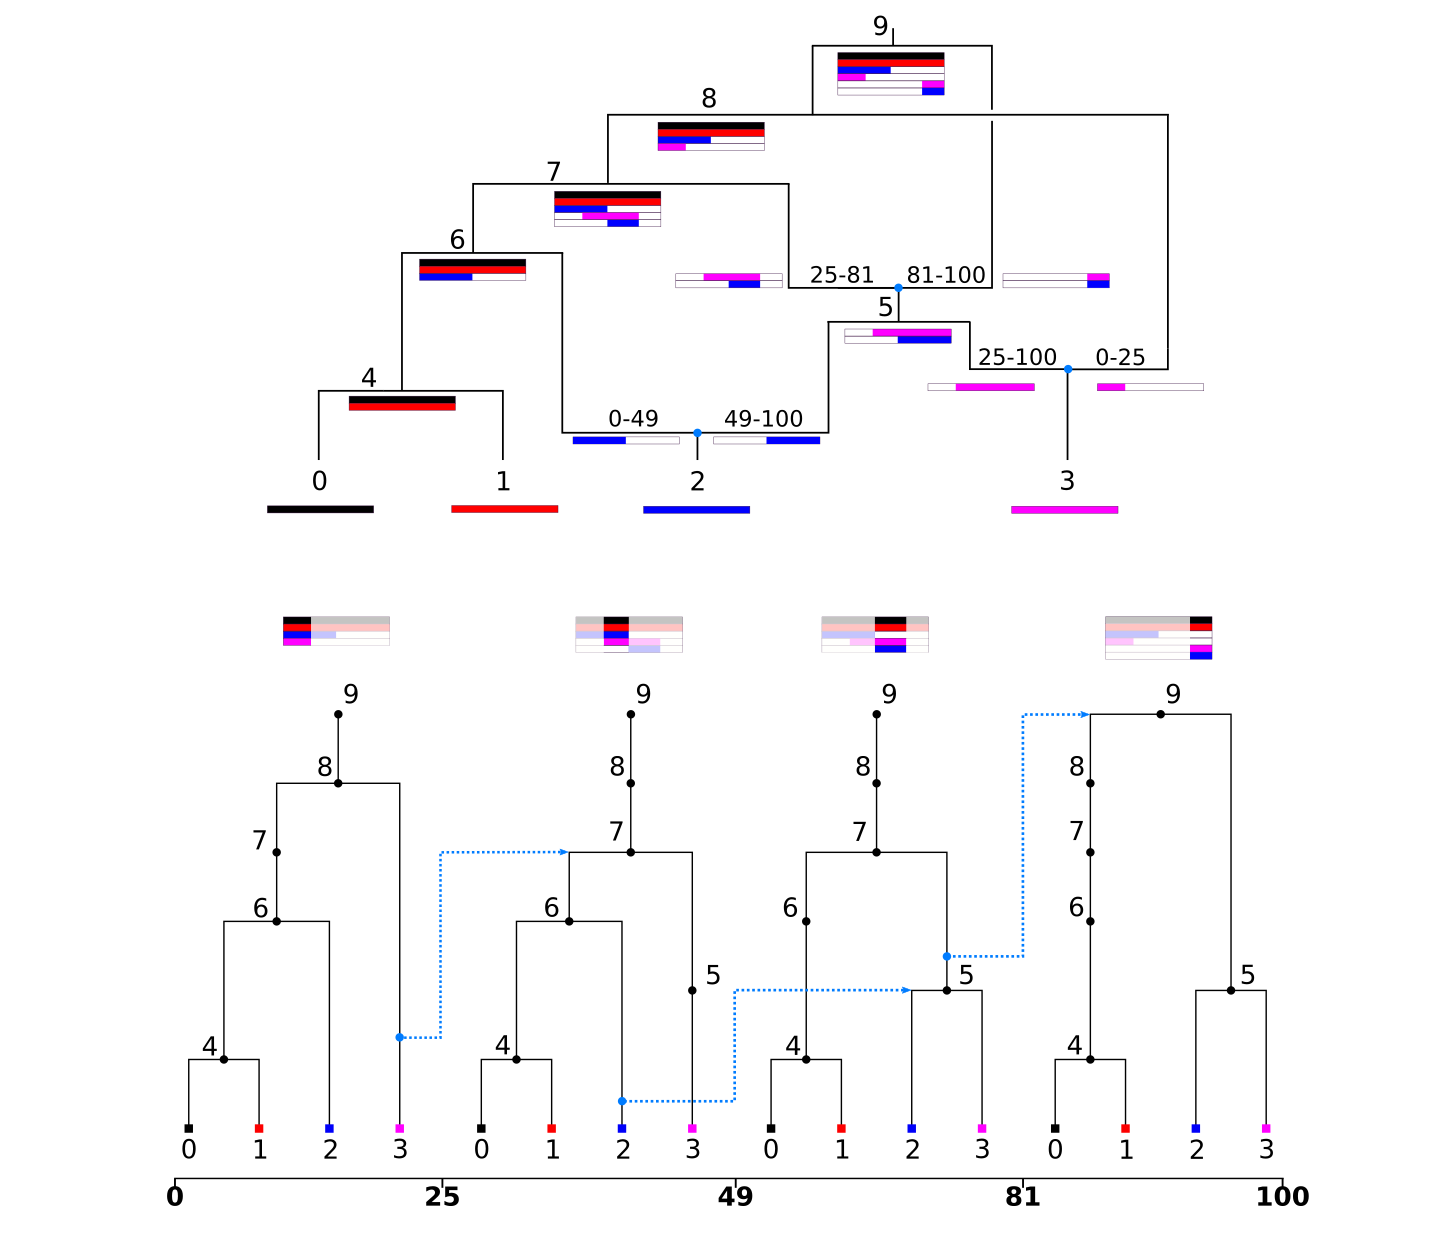
\includegraphics[width=\textwidth]{figures/smc_custom_2rows.png}
\caption{ARG (top left) generated under the SMC and its representation as a 
series of local trees. The presence of the unary nodes in the local trees 
ensure these two representations contain the same information. 
The ARG is augmented with haplotype information, coloured according to the 
samples that inherit from it. 
Note how the presence of a unary node on a local tree is 
indicative of either a past (to the left of the local tree) 
or future (to the right) coalescence event. It therefore modifies the 
left-to-right logic of the SMC whereby the floating lineage coalesces randomly
with a the remaining portion of the local tree. 
}
\label{fig:smc-unary}
\end{figure}



\subsection{Calculating likelihoods} \label{par:liks}

Retracing the ARG backwards in time, each coalescence event is associated with two child 
lineages, $c$ and $d$, and a single parent, $p$. By defining $C_i(t)$ asymmetrically, 
the history of each these two child lineages can be considered independently without 
risking to double count any of the coalescence events. The likelihood of 
observing the edge $(c, p, X_{cp})$ can thus be considered independently from 
the likelihood of all other edges, and in particular from the likelihood 
of $(d, p, X_{dp})$.\\

% extends from here means min(X_{cp})=x, max(X_{cp})=y
% improve this description here
Assuming $(c, p, X_{cp})$ extends from $x$ to $y$ along the genome and $t_i$ 
indicates the age of 
node $i$ in the ARG, then the probability of not observing a recombination across the 
entire area (span x depth) of this edge is 

% full extent of segment
\begin{equation}\label{eq:span}
A_{(c, p)}(\theta) = e^{-r (y-x)(t_p - t_{c})}
\end{equation}
% also x and y not necessarily equal to x_{c_{1}0} and y_{c_{1}m}.

What's left to compute the likelihood, is to take into account all events 
associated with $x$, 
the leftmost coordinate of $(c, p, X_{cp})$. This is either only the 
coalescence event involving 
$c$ and $d$. In this case $x=x_{c0}$. Or, $x$ can a new recombination break point that 
occurred on the lineage represented by $c$ at some time $s$ between $t_{c}$ 
and $\min(t_p, t_{p^{\prime}})$, where $p^{\prime}$ is the parent of the 
edge $(c, p^{\prime}, X_{cp^{\prime}})$ ending at $x$.
In the latter case the new lineage starting at $x$ can be given a temporary label 
$c^{\prime}$ such that with the same logic from the previous paragraph we 
can define $F(c^{\prime}, s, t) = \int_{s}^{t} I_{c^{\prime}}(u)du$. 

\begin{equation}\label{eq:depth}
B_{(c, p)}(\theta) = \begin{cases}
e^{-\lambda F(c, t_c, t_p)} \lambda^{I_{cd}(t_p)} & x=x_{c0} \\
\int_{t_c}^{t_{p} \wedge t_{p^{\prime}}} r e^{-rs} e^{-\lambda F(c^{\prime}, s, t_{p})} ds \lambda^{I_{c^{\prime}d}(t_p)} & x=x_{c^{\prime}0}>x_{c0} \\
\end{cases}
\end{equation}

Here, the (second) exponential term gives the probability of not observing a 
coalescence event before $t_p$. In case of a recombination, $re^{-rs}$ further 
gives the probability of observing a recombination 
at time $s$ given a Poisson process along position $x$ with rate $r$. The 
time of the recombination is integrated out.
The last term gives the point probability density of the coalescence event 
that terminates the edge. The indicator function is used to resolve 
the non-reciprocal nature of coalescence events as defined here.\\

The likelihood of ARG $\mathcal{G}$ defined by the set of edges $E$ and
given parameters $\theta$ then is

\begin{equation}\label{eq:full-lik}
\mathcal{L}(\mathcal{G}|\theta) = \prod_{(c, p) \in E} A_{(c, p)}(\theta) * B_{(c, p)}(\theta)
\end{equation}

% Does this hold for the case beyond the root of the genealogy?

[TO DO: improve this remark: when recording an ARG we do record edges in this situation,
however, msprime simulations will stop recording edges for local trees that have reached 
their local mrca.] 
Because the likelihood is computed based on edges,
and edges are no longer recorded once the local most recent common ancestor 
has been reached, we will underestimate the number of positions where 
a recombination could have occurred in case a recombination hits a 
lineage with trapped non-ancestral material (see end \ref{par:description}). 
If we assume that only a single recombination could have  
occurred, then it suffices however to provide a correction factor $g$ in equation
\ref{eq:depth}. Here $g$ represents the 
length of non-ancestral material along which a recombination would have resulted  
in the same observed local sequence of tree changes.\\


\begin{figure}[!ht] \label{fig:algo}
\centering
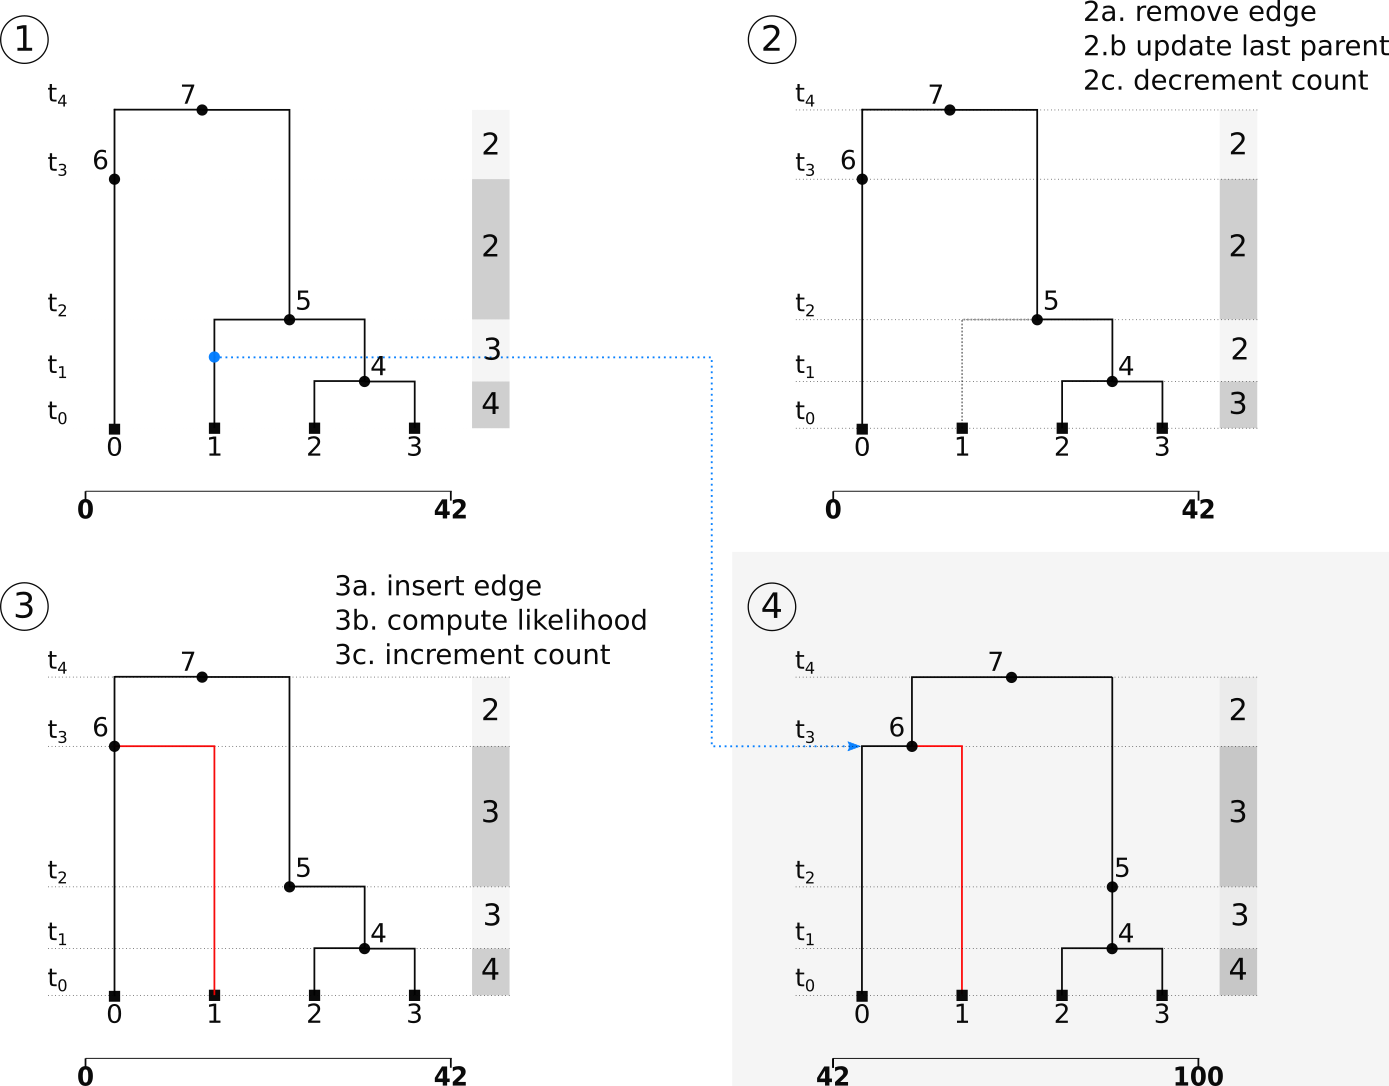
\includegraphics[width=\textwidth]{figures/ts_algo_2rows.png}
\caption{Description of algorithm: Moving along the genome we transition from  
local tree $T_1$ (1) to the next, $T_2$ (4). Edges that do not persist in $T_2$ are 
removed (2). Edges starting at the left coordinate of $T_2$ are inserted (3). 
After deletion or insertion of an edge the count vector $I$ is updated along the 
corresponding internode intervals. Prior to updating $I$ following an insertion, 
the likelihood for that edge is computed as $I$ then represents the total number of 
lineages the lineage associated with this new edge can 
coalesce with. By moving along the genome in this way, each edge gets visited exactly once.}
\end{figure}

Note that we are only considering the topology and branch length information of any ARG. 
Extending this expression by adding the likelihood of observing a set of mutations 
given an ARG is straightforward.


\subsection{Tree sequence format} \label{par:algo}

Although the argument outlined in the previous paragraph is valid for any ARG, here we 
will describe how to (efficiently) extract the information required to associate a
tree sequence encoding of an ARG with a likelihood under the SMC (see fig. \ref{fig:smc-unary}).\\

Formally, we represent a tree sequence using a set of tables \citep{kelleher_efficient_2018}. 
This simple tabular representation of any ARG $\mathcal{G} = (N, E)$, can be 
augmented with additional tables with information on sequence variation
using a site and mutation table. The node table stores information on all 
haplotypes $N$ in the tree sequence. Information about how nodes relate to 
each other along the genome is defined in a tabular encoding of $E$.
Each row in this edge table constitutes a tuple \texttt{(left, right, parent, child)}.
Note that we defined the extent of any edge $\epsilon \in \mathcal{G}$ as the union of 
disjoint intervals. In the tree sequence encoding however, $\epsilon$ will be represented 
by a single entry for each contiguous interval. As remarked before, under the SMC, this 
distinction only matters beyond the root of the genealogy. The distinction between both 
types of edges will therefore not be made in the remainder of the paper.
% Although it does requires us to keep track of some additional information to avoid
% wrongfully assuming a recombination event happened.
% Similarly, the distinction between the lineage associated with an edge, and the edge 
% itself can render things very verbose.
\\

The likelihood computation as described above can be done with a single pass 
of the edge table.
The central problem however is to efficiently maintain the state $I_e(t)$, which counts 
the number of lineages (the lineage associated with) the focal edge $\epsilon$ can coalesce 
with at time $t$. 
The definition of $I_{kl}$ (\ref{def:coal}) is based on the assumption 
that we can impose a strict total order on all (overlapping) lineages based on their 
starting point. The tree sequence encoding provides us with a natural order on all lineages.  
For each local tree with left coordinate $x$, lineages associated with an edge 
starting at $x$ can only coalesce with the subset of lineages associated with one of the
edges that make up that local tree. Each of these edges will either already have 
been present in the previous local tree, or will have the same starting point $x$.
In \texttt{tskit}, the order in which edges are inserted and removed 
while moving from one tree to the next, is determined by the index 
vectors $\textbf{i}$ and $\textbf{o}$ \citep{kelleher_efficient_2016}.
The edge insertion vector $\textbf{i}$ gives the ordering of edges sorted by left 
endpoint, and among edges with the same left endpoint, sorted so that edges closer 
to the root appear later. The edge removal vector $\textbf{o}$ is similar, 
except gives the ordering of edges by right endpoint and with edges closer to the 
root appearing sooner. The variables $\texttt{i}$ and 
$\texttt{o}$ are used to keep track of our position in the edge insertion and edge removal 
indexes as we move along the tree sequence. This order imposes the 
strong ordering on all edges as required by the definition of $I_{kl}$.\\

% edge diff algorithm
The size of the subset of lineages in each internode interval each lineage 
can coalesce with can thus be maintained by keeping track of a single vector $I$ 
that is decremented or incremented as defined by
$\textbf{o}[\texttt{o}]$ and $\textbf{i}[\texttt{i}]$, 
Further keep track of a last-parent array to detect recombination events.
We can thus compute a likelihood for the tree sequence, while visiting each edge only once.

More concretely, prior to inserting an edge, $I$ represents the number of lineages 
the lineage associated with 
that edge can coalesce with. Then insert the edge and update the counts.

To transition from one tree to the next, we first iterate across the indices of all edges 
in $\textbf{o}$ from its current index up to $\texttt{o}$. For each edge in we decrement $I$ 
from index \texttt{edge.child} to \texttt{edge.parent}. We subsequently iterate across the 
edges in $\textbf{i}$ up to index $\texttt{i}$. For each new edge, we first compute the likelihood 
associated with that edge and then 
increment $I$ from \texttt{edge.child} to \texttt{edge.parent}.\\

% ADD IN RESULTS
Figure \ref{sup:fig:vs-argweaver} shows the expected near-perfect correlation 
between the coalescent prior as returned by \argweaver and the likelihood as computed here. 
We simulated 1Mb of data for 10 diploid individuals 
under the SMC using human-like parameters. 100 samples were taking from the posterior every for 
a total of 1000 MCMC iterations.
 

\subsection{Flexibility / general class of ARGs}

% slicing of the ARG
By explicitly associating a single likelihood with each edge, we can compute a likelihood 
under the SMC for any valid tree sequence. The \texttt{tskit} library provides a whole range  
of subsetting operations on tree sequences allowing us to slice the ARG in time and/or space, 
as well as reduce the number of tracked samples. 
Any such subset of the tree sequence is itself a valid tree sequence 
that can again be used to compute a likelihood with. Our approach therefore strenghtens 
the inherent ability of ARGs to provide us with temporal 
resolution on the inferred genealogical history of a sample. 
We can further readily incorporate changes in $N_e$ and $r$, 
both in time as well as along the genome by respectively adding intervals to $I$ 
or by splitting edges when/wherever the parameter set changes.
[NOTE: these options have already been implemented in the current implementation]

Although we rely heavily on unary nodes to provide us with the necessary 
information on recombination events, our algorithm only implicitly assumes there presence.
The algorithm can therefore also accomodate for 
those inferred ARGs that lack unary nodes (e.g.\ \relate). 
Note that without unary nodes, our algorithm will detect a recombination event along 
both coalescing lineages in case of a (sub)tree height changes along the ARG as both 
edges would switch parent nodes. This can be mitigated by limiting the number of 
'inferrable' recombination events per coalescence event to 1.
% simulated results
We simulated 1000 ARGs under the Hudson coalescent retaining all recombination information 
and computed the corresponding likelihood using \texttt{msprime} \citep{baumdicker_efficient_2021}. 
After removing the recombination nodes the likelihoods as defined here were computed both with and 
without the unary nodes. Figure \ref{sup:fig:vs-hudson} shows that the proportion of variation 
explained is higher when the unary nodes are retained.

% polytomies
[TO DO: polytomies] The above algorithm treats each edge independently which implies 
we can deal with polytomies.
[TO DO: discuss, what if the identity of internal nodes is not preserved across trees]
 
\section{Discussion}

Here, we have introduced a scalable algorithm to compute likelihoods 
under the SMC for a general class of ARGs. By formulating the SMC backwards in time 
we were able to associate a single likelihood value with each edge in the ARG. 
The compatibility of the algorithm with the \texttt{tskit} library allows us to 
exploit its associated efficiencies both for the current work and its future 
applications. This work will contribute significantly 
to ARG-based analysis becoming a standard part of the population 
and statistical genetics toolkit. 
In particular, we see three main applications for the work presented here. 
Firstly, the ability to associate inferred ARGs with a likelihood given a demographic 
model and an associated set of parameters will help bridge the gap between the tremendous recent 
advances in ARG inference and the current state of the art statistical inference of 
past demography. Secondly, hybrid ARG-inference methods that combine the best of both 
heuristic and model-based inference approaches are now possible.
Thirdly, using a model we can quantify the uncertainty inherently associated 
with ARG-reconstruction.

% 1/ statistical inference
Currently most/all ARG-based inference methods base their analysis on marginal 
trees \citep{hejase_2022} [TO DO: add more refs]. The theory and associated algorithm 
provided here can function as a building block of a 
demography-aware genealogy sampler that would allow us to incorporate the information 
provided by recombination events.
More concretely, given our algorithm, any inferred ARG can be used a good starting point 
for a future MCMC-sampler. This potentially implies a massive runtime reduction by 
reducing the necessary burn-in period. Furthermore, by integrating out the exact time 
to the recombination event we further restrict the size of the ARG space that needs to 
be explored. This MCMC-sampler would again rely on the tree sequence data structure to 
efficiently generate and evaluate any new proposal (see \citep{mahmoudi_bayesian_2022}). 
$N_e$-changes as well as multiple populations and migration can be readily incorporated 
in the current algorithm.\\


% 2/ hybrid ARG-inference
Hybrid backwards-in-time simulations that combine Wright-Fisher dynamics in the 
very recent past and coalescent simulations for the remaining time are a tried and tested 
approach \citep{bhaskar_distortion_2014, nelson_accounting_2020} to enable large scale 
simulations while avoiding the documented biases of the coalescent relative to the 
Wright-Fisher model \citep{bhaskar_distortion_2014, wakeley_gene_2012}. The same approach 
could be used for ARG-inference where one can rely on a heuristic inference method for 
the recent past, while using a model-based approach beyond that cutoff point.\\

% 3/ quantifying uncertainty [unfinished]
Both of these future directions tie in with the desired ability of any ARG-related method to 
quantify the uncertainty associated with 


to quantify uncertainty by sampling 
from an underlying distribution. 

This will in particular enable us to deal with those 
parts in both time and along the genome for which we have insufficient information to confidently 
reconstruct the ARG. The presence of polytomies in ARGs inferred by \tsinfer, for example, 
represents uncertainty. Systematicallty breaking them by sampling from the coalescent rather 
then randomly would already be a major step forward. 


Quantifying uncertainty would not necessarily always have to be associated 
with sampling 
with dealing with the entire subset of all compatible genealogies. Uncertainty could also 
be quantified and passed on as metadata to a parent node representing the uncertainty 
in the interval spanned by the polytomy.
% can something similar be done for stacked recombinations?

[TO DO] Comment on accuracy. The described algorithm has been implemented in such a way that 
any valid tree sequence will result in a likelihood value. This also holds for any tree sequence 
that does not meet the assumptions. We see it as future work to determine to what extent 
particular deviations from these assumptions will affect the shape of the likelihood surface given 
a set of parameters.

% final conclusion


\section{Data availability}

All scripts and data used for this manuscript are available on https://github.com/gertjanbisschop/smc-bit-paper
An implementation of the algorithm is available on https://github.com/gertjanbisschop/runsmc.

\bibliographystyle{plainnat}
\bibliography{paper.bib, temp.bib}

\pagebreak 

\supplementarysection
\section*{Supplementary Information}


\begin{figure}[!ht]
\centering
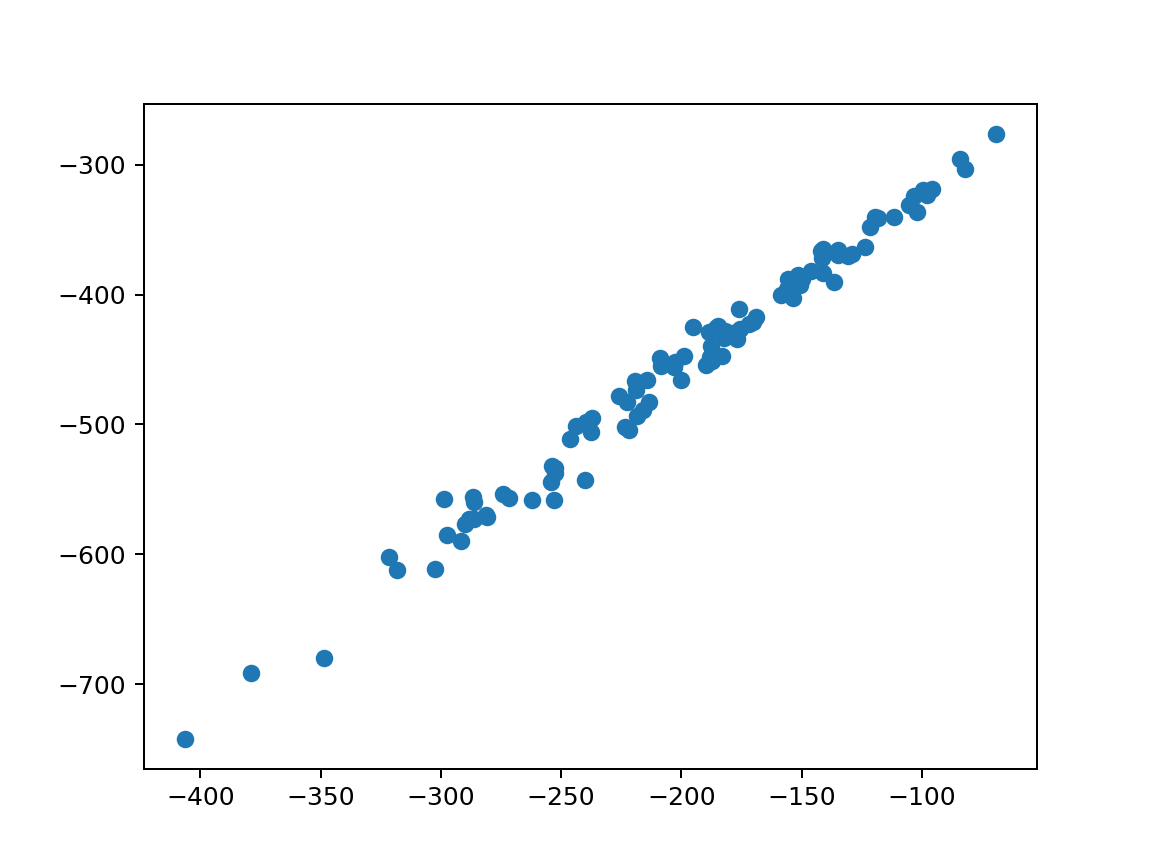
\includegraphics[width=0.75\textwidth]{figures/supplementary-figs/argweaver_vs_runsmc.png}
\caption{Compare likelihoods inferred ARGs ARGweaver: placeholder for final figure with similar content}
 \label{sup:fig:vs-argweaver}
\end{figure}


\begin{figure}[!ht]
\centering
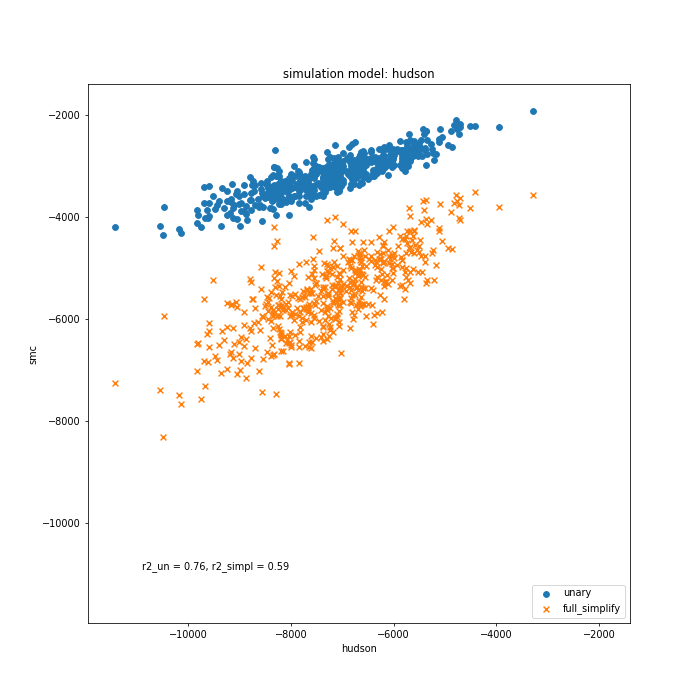
\includegraphics[width=0.75\textwidth]{figures/supplementary-figs/v_hudson_unary_simpl.png}
\caption{Compare likelihoods Hudson and SMC with and without unary nodes: placeholder for final figure with similar content}
\label{sup:fig:vs-hudson}
\end{figure}

\end{document}
